\section{Results}
\label{sec:results}

\subsection{Routing reveals reasoning-state information beyond text}
\label{sec:readout-results}

Routing information gain (RIG) is positive in all eight evaluated models, improving held-out present-state prediction beyond the retrospective text baseline (Figure~\ref{fig:readout}).
%
RIG ranges from 0.079 to 0.149 nats per sentence on the common 522-question, 509-family population.
%
GPT-OSS has a mean reduction of \cid{0.0786}{0.0168}{0.0171} nats, and Gemma has a reduction of \cid{0.1487}{0.0117}{0.0127} nats.
%
Each model-specific corrected interval excludes zero.
%
Appendix~\ref{app:readout} gives the complete signed contrasts and sentence counts.
%

\begin{figure}[tb]
\centering
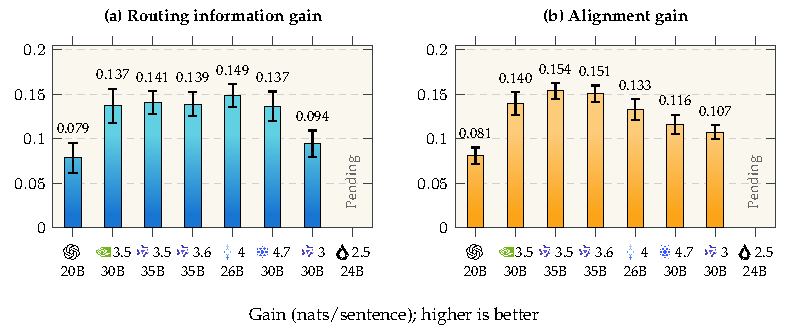
\includegraphics[width=\linewidth]{figures/journal/readout.pdf}
\caption{Routing information gain (RIG) over text in panel (a) and alignment gain over the lexical null in panel (b), in nats per sentence on a common scale.
%
Positive bars favor observed routing.
%
Horizontal labels give the mean gains.
%
Whiskers show the model-specific seven-comparison 95\% family-bootstrap intervals after reversing the loss-contrast sign.}
\label{fig:readout}
\end{figure}

The lexical-null comparison retains the same direction in every model.
%
Its original corrected gain intervals also exclude zero.
%
Thus the readout gain depends on information retained by the original routing alignment beyond the declared token and absolute-position stratification.
%
The baseline includes the current sentence and its available neighbours, so the gain reflects additional routing information.
%

This common direction supports reasoning-label information in sparse computation across several routing geometries.
%
The magnitude remains conditional on each model's generated text, available labels, and representation.
%
Comparing two gains is therefore not a controlled test of which architecture contains more interpretable reasoning.
%
The result establishes the increment within the specified prediction task.
%

\subsection{State balancing exposes a coverage trade-off}
\label{sec:selection-results}

State-balanced retention achieves higher weakest-state coverage (WSC) than labelled frequency in GPT-OSS, Nemotron, Gemma, GLM, Qwen3-30B, and LFM2.5 (Table~\ref{tab:selection}).
%
The direction holds in all five folds for each of these models.
%
Nemotron has the largest mean coverage gain, $\Delta\mathrm{WSC}=4.58$ percentage points, improving minimum coverage from 78.63\% to 83.22\%.
%
LFM2.5 improves by 3.46 points, GLM by 2.79 points, and GPT-OSS by 1.77 points.
%
These results show that the least-covered reasoning class can benefit from giving classes equal weight during expert selection.
%

% Adapted from SPSD tab:main-results and SYNCO tab:mainRes.
\begin{table}[tb]
\centering\small
\caption{Weakest-state coverage (WSC): the mean minimum held-out native selected-slot coverage across reasoning classes (\%) at 75\% expert retention.
%
Entries average the five family folds.
%
$\Delta\mathrm{WSC}$ is balanced minus frequency in percentage points.
%
Bold and underline mark the highest and second-highest selector means within each model.
%
The subscript n/e means that a 95\% confidence interval was not estimated in the saved outputs.
%
Individual values appear in Table~\ref{tab:selection-folds}.}
\label{tab:selection}
\setlength{\tabcolsep}{2.5pt}
\begin{adjustbox}{max width=\linewidth}
\begin{tabular}{@{}lrrrr@{}}
\toprule
 & \multicolumn{3}{c}{WSC (\%) $\uparrow$} & $\Delta\mathrm{WSC}$ (pp) \\
\cmidrule(lr){2-4}
Model & Balanced & Frequency & Random & Balanced $-$ frequency \\
\midrule
\modelname{openai}{GPT-OSS-20B} & $\mathbf{96.78}_{\mathrm{n/e}}$ & $\underline{95.01}_{\mathrm{n/e}}$ & $77.14_{\mathrm{n/e}}$ & $+1.77_{\mathrm{n/e}}$ \\ 
\modelname{nvidia}{\shortstack[l]{Nemotron-3.5-Lightning\\30B-A3B}} & $\mathbf{83.22}_{\mathrm{n/e}}$ & $\underline{78.63}_{\mathrm{n/e}}$ & $75.32_{\mathrm{n/e}}$ & $+4.58_{\mathrm{n/e}}$ \\ 
\modelname{qwen}{Qwen3.5-35B-A3B} & $\underline{91.62}_{\mathrm{n/e}}$ & $\mathbf{92.96}_{\mathrm{n/e}}$ & $75.09_{\mathrm{n/e}}$ & $-1.35_{\mathrm{n/e}}$ \\ 
\modelname{qwen}{Qwen3.6-35B-A3B} & $\underline{93.23}_{\mathrm{n/e}}$ & $\mathbf{93.78}_{\mathrm{n/e}}$ & $74.89_{\mathrm{n/e}}$ & $-0.55_{\mathrm{n/e}}$ \\ 
\modelname{gemma}{Gemma-4-26B-A4B} & $\mathbf{99.42}_{\mathrm{n/e}}$ & $\underline{99.20}_{\mathrm{n/e}}$ & $74.53_{\mathrm{n/e}}$ & $+0.21_{\mathrm{n/e}}$ \\ 
\modelname{zhipu}{GLM-4.7-Flash (30B-A3B)} & $\mathbf{89.28}_{\mathrm{n/e}}$ & $\underline{86.49}_{\mathrm{n/e}}$ & $74.04_{\mathrm{n/e}}$ & $+2.79_{\mathrm{n/e}}$ \\ 
\modelname{qwen}{Qwen3-30B-A3B} & $\mathbf{98.79}_{\mathrm{n/e}}$ & $\underline{98.21}_{\mathrm{n/e}}$ & $73.38_{\mathrm{n/e}}$ & $+0.59_{\mathrm{n/e}}$ \\ 
\modelname{liquid}{LFM2.5-24B-A2B} & $\mathbf{92.56}_{\mathrm{n/e}}$ & $\underline{89.10}_{\mathrm{n/e}}$ & $74.52_{\mathrm{n/e}}$ & $+3.46_{\mathrm{n/e}}$ \\ 
\bottomrule
\end{tabular}
\end{adjustbox}
\end{table}


Qwen3.5 and Qwen3.6 reverse this pattern.
%
Frequency has higher minimum coverage in every fold, by mean differences of 1.35 and 0.55 points, respectively.
%
This reversal occurs under the same training families, layer quotas, tie-breaking rule, and evaluation endpoint.
%
Equal class weight consequently does not supply a uniformly better allocation rule.
%
The coverage advantage of a selector depends on how class-specific allocation differs from the model's pooled labelled frequency.
%

\begin{figure}[tb]
\centering
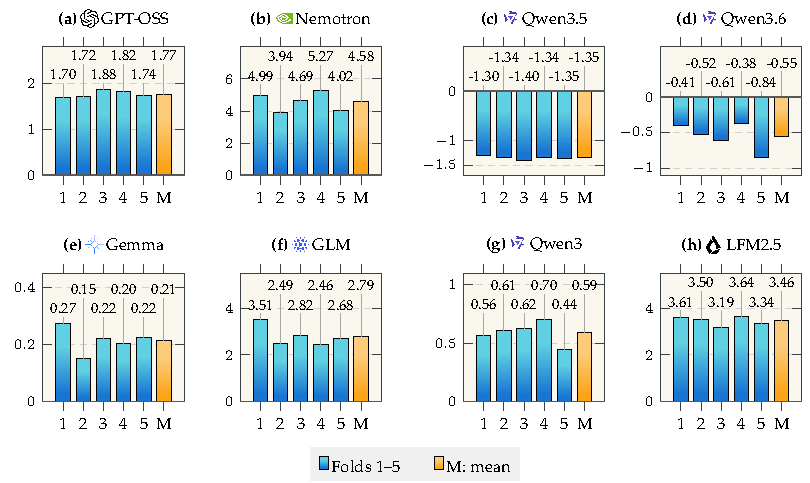
\includegraphics[width=\linewidth]{figures/journal/selection.pdf}
\caption{Gain in weakest-state coverage (WSC) at 75\% expert retention.
%
Positive values favor state balancing over labelled frequency.
%
Each model panel shows five fold-specific differences and their mean (M) in percentage points (pp), with model-specific vertical scales.}
\label{fig:selection}
\end{figure}

Gemma and Qwen3-30B retain 99.42\% and 98.79\% minimum class coverage under balancing.
%
Their mean gains over frequency are only 0.21 and 0.59 points, consistent with little remaining room for coverage improvement at this budget.
%
Nemotron retains a substantially smaller fraction under either learned selector, even though its balancing gain is larger.
%
Near-complete coverage indicates concentrated native allocation.
%
The paired difference measures the effect of changing the selection rule.
%

The fixed random masks have minimum coverage between 73.4\% and 77.2\% across model--fold cells.
%
Both learned methods improve on these masks in the reported mean comparison.
%
Their random baseline conditions on one set of priorities per model.
%
It does not estimate variation over independently sampled random masks.
%
All 120 model--fold--method cells are retained in Appendix~\ref{app:selection}.
%
The five folds partition test families, but their training sets overlap, so their spread supplies a stability description rather than five independent replications.
%

\subsection{Observed reasoning concentrates on analysis and implementation}
\label{sec:dynamics-results}

Implementation and analysis occupy most of the observed labelled tokens in every evaluated model (Figure~\ref{fig:occupancy}).
%
Implementation ranges from 31.18\% in GLM to 45.28\% in Gemma.
%
Analysis ranges from 24.38\% in Qwen3-30B to 31.76\% in Qwen3.5.
%
In contrast, monitoring occupies 2.79--8.17\% and verification 10.11--15.66\%.
%
These unequal shares explain why pooled labelled frequency and equal-class selection need not rank experts uniformly across reasoning activities.
%

\begin{figure}[tb]
\centering
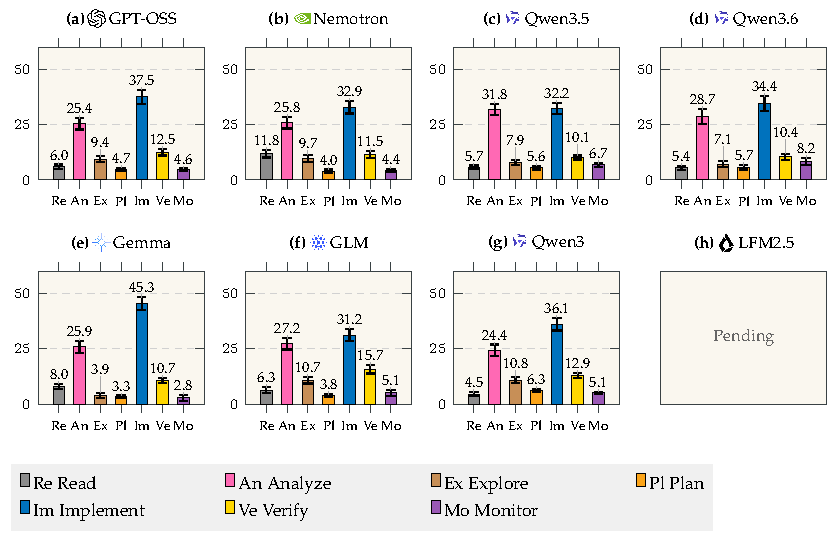
\includegraphics[width=\linewidth]{figures/journal/occupancy.pdf}
\caption{Seven reasoning-state occupancies among observed labelled tokens, shown in model panels on a common percentage scale.
%
Horizontal labels give means.
%
Whiskers show simultaneous 95\% confidence intervals within each model's native-dynamics panel, using 10,000 whole-family resamples.
%
Benchmarks and supported families receive equal weight.
%
Qwen3.6 uses 509 families.
%
The other evaluated models use 1,486.}
\label{fig:occupancy}
\end{figure}

The native summaries also quantify how much of the completion receives an observed label (Table~\ref{tab:label-coverage}).
%
Coverage ranges from 7.80\% for Qwen3.6 to 28.16\% for GPT-OSS under this equal-benchmark, equal-family estimand.
%
The occupancy comparison therefore describes the labelled part of the trace.
%
It cannot recover the classes of the remaining tokens or identify the complete temporal structure of a solution.
%
Qwen3.6 additionally has a smaller population in this analysis, so its distribution should be read with that support.
%


The complete seven-state distributions and their intervals appear in Appendix~\ref{app:dynamics}.
%
Variation in annotation coverage and the generated solutions is part of the comparison.
%
The displayed ordering of occupancy estimates supplies a descriptive pattern, while a claim about a difference between models would require a corresponding paired cross-model contrast.
%

\subsection{Verification entry differs from persistence}
\label{sec:transition-results}

The transition matrices expose how an observed activity connects to its next labelled sentence (Figure~\ref{fig:state-transitions}).
%
Implementation continues into another implementation sentence with mean probability \cid{48.61}{5.04}{5.04}\% in GPT-OSS and \cid{54.53}{6.70}{6.70}\% in Gemma.
%
The large implementation occupancy therefore accompanies substantial within-state persistence.
%
Moving from implementation to verification has mean probability \cid{17.27}{4.27}{4.27}\% in GPT-OSS and \cid{20.33}{4.81}{4.81}\% in Qwen3-30B (Table~\ref{tab:state-transitions}).
%
Repeating verification is more common than entering it from implementation in every evaluated model's point estimates.
%
This distinction separates access to a checking activity from persistence once it has started.
%
The overlapping model-specific intervals do not establish a cross-model ordering.
%

\begin{figure}[tb]
\centering
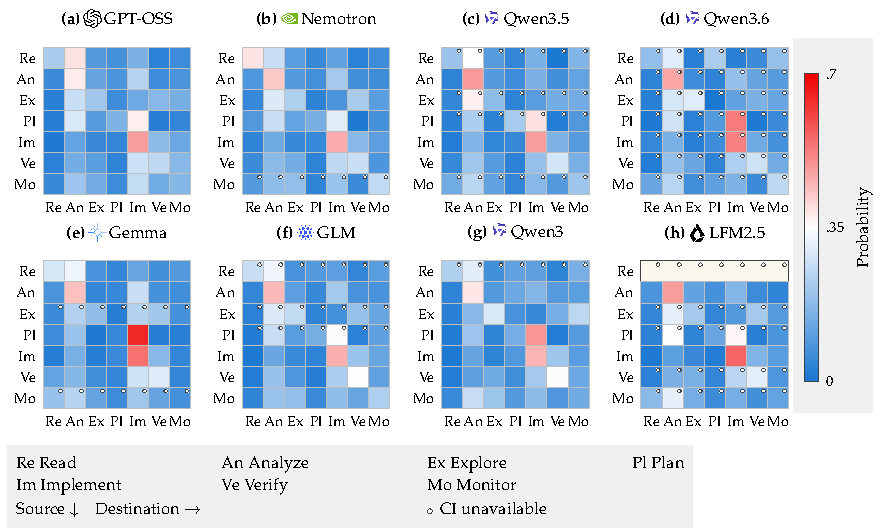
\includegraphics[width=\linewidth]{figures/journal/state_transitions.pdf}
\caption{Observed reasoning-state transitions in the eight evaluated models.
%
Rows denote the current state and columns the next adjacent labelled sentence.
%
Each row sums to one.
%
Colors encode saved equal-benchmark, equal-family mean probabilities on a common blue-to-red scale from 0 to 0.7.
%
Hollow corner marks identify cells whose original model-specific simultaneous 95\% whole-family-bootstrap interval is unavailable, including all Qwen3.6 transition cells and the sparsely supported LFM2.5 cells.
%
Missing-label gaps are not bridged.
%
Qwen3.6 uses 509 families.
%
Other evaluated models use 1,486.
%
Table~\ref{tab:state-transitions} gives selected means and confidence limits, and Appendix~\ref{app:dynamics} expands the duration comparison.}
\label{fig:state-transitions}
\end{figure}

% Native SYNCO tab:mainRes grouped diagnostic columns and caption-only key.
% Complete label-coverage and transition tables merged on identical model identity.
% Source: native_dynamics.json, unchanged saved means and interval endpoints.
\begin{table}[tb]
\centering\small
\caption{Annotation coverage and native state dynamics, with whole-family-bootstrap, model-specific simultaneous 95\% confidence intervals as subscripts.
%
Coverage is the labelled fraction of completion tokens.
%
Transition probabilities condition on the current state and next observed sentence boundary.
%
Missing-label gaps are not bridged.
%
Benchmarks and supported families receive equal weight.
%
Verify dwell includes contiguous labelled runs censored by coverage boundaries.
%
Qwen3.6's three transition intervals and LFM2.5's Verify persistence interval are unavailable under the saved support gate.
%
\textrm{An}, \textrm{Im}, and \textrm{Ve} denote Analyze, Implement, and Verify; n/e marks an unestimated interval.}
\label{tab:state-transitions}\label{tab:label-coverage}
\setlength{\tabcolsep}{2.5pt}
\begin{adjustbox}{max width=\linewidth}
\begin{tabular}{@{}lrccccc@{}}
\toprule
 & \multicolumn{2}{c}{Annotation} & \multicolumn{3}{c}{Transitions (\%)} & Dwell \\
\cmidrule(lr){2-3}\cmidrule(lr){4-6}\cmidrule(lr){7-7}
Model & Families & Coverage (\%) & \textrm{An} $\to$ \textrm{Im} & \textrm{Im} $\to$ \textrm{Ve} & \textrm{Ve} $\to$ \textrm{Ve} & \textrm{Ve} (tokens) \\
\midrule
\modelname{openai}{GPT-OSS-20B} & 1,486 & \cid{28.16}{0.93}{0.93} & \cid{24.17}{6.03}{6.03} & \cid{17.27}{4.27}{4.27} & \cid{25.29}{6.17}{6.17} & \cid{16.18}{1.06}{1.06} \\
\modelname{nvidia}{\shortstack[l]{Nemotron-3.5-Lightning\\30B-A3B}} & 1,486 & \cid{20.83}{1.17}{1.17} & \cid{21.31}{6.37}{6.37} & \cid{16.90}{4.93}{4.93} & \cid{26.73}{7.90}{7.90} & \cid{21.05}{1.96}{1.96} \\
\modelname{qwen}{Qwen3.5-35B-A3B} & 1,486 & \cid{8.06}{0.26}{0.26} & \cid{14.79}{5.22}{5.22} & \cid{15.43}{5.96}{5.96} & \cid{28.43}{9.90}{9.90} & \cid{14.35}{1.24}{1.24} \\
\modelname{qwen}{Qwen3.6-35B-A3B} & 509 & \cid{7.80}{0.39}{0.39} & $18.78_{\mathrm{n/e}}$ & $13.32_{\mathrm{n/e}}$ & $27.63_{\mathrm{n/e}}$ & \cid{13.67}{1.49}{1.49} \\
\modelname{gemma}{Gemma-4-26B-A4B} & 1,486 & \cid{16.27}{0.58}{0.58} & \cid{26.56}{6.57}{6.57} & \cid{16.89}{4.10}{4.10} & \cid{29.86}{8.36}{8.36} & \cid{17.95}{1.33}{1.33} \\
\modelname{zhipu}{GLM-4.7-Flash (30B-A3B)} & 1,486 & \cid{16.79}{1.22}{1.22} & \cid{21.13}{6.58}{6.58} & \cid{19.92}{6.71}{6.71} & \cid{34.54}{8.76}{8.76} & \cid{21.12}{1.33}{1.33} \\
\modelname{qwen}{Qwen3-30B-A3B} & 1,486 & \cid{15.90}{0.80}{0.80} & \cid{16.28}{4.73}{4.73} & \cid{20.33}{4.81}{4.81} & \cid{34.26}{6.83}{6.83} & \cid{16.53}{1.69}{1.69} \\
\modelname{liquid}{LFM2.5-24B-A2B} & 1,486 & \cid{9.96}{0.82}{0.82} & \cid{16.21}{7.70}{7.70} & \cid{15.83}{6.37}{6.37} & $30.61_{\mathrm{n/e}}$ & \cid{16.39}{2.04}{2.04} \\
\bottomrule
\end{tabular}
\end{adjustbox}
\end{table}


Observed verification runs also differ in duration.
%
Their mean token length is \cid{21.12}{1.33}{1.33} in GLM and \cid{13.67}{1.49}{1.49} in Qwen3.6.
%
Longer dwell can represent a sustained check, repeated checking, or a boundary introduced by sparse annotation.
%
It does not by itself identify wasted computation.
%
Routing guidance must therefore consider the candidate being checked and the usefulness of its continuation, alongside the state sequence.
%
These summaries describe the annotated segments, rather than a complete uncensored reasoning process.
%

\subsection{Routing anticipates the next reasoning state}
\label{sec:next-results}

The prospective comparison finds additional next-state information in GPT-OSS and Qwen3.6 (Figure~\ref{fig:next-state}).
%
The mean anticipatory routing gains (ARG) are \cid{0.02073}{0.00472}{0.00475} nats per pair for GPT-OSS and \cid{0.05570}{0.01417}{0.01374} for Qwen3.6.
%
The respective adjacent-pair populations contain 509 and 494 questions.
%

\begin{figure}[tb]
\centering
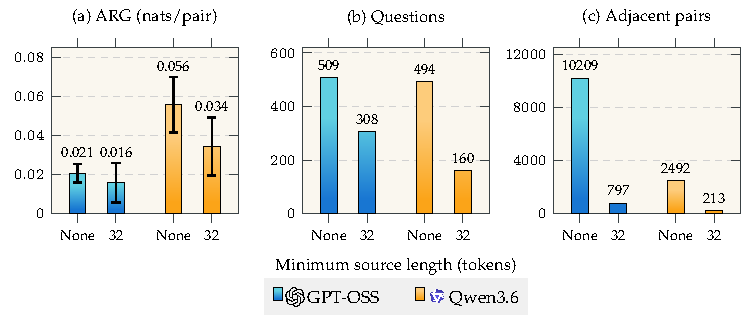
\includegraphics[width=.98\linewidth]{figures/journal/next_state.pdf}
\caption{Anticipatory routing gain and evaluation support under source-length restriction.
%
(a) ARG from trailing 16-token routing features; (b) contributing questions; (c) adjacent pairs.
%
None imposes no minimum source length; 32 requires at least 32 source tokens.
%
Positive ARG favors routing beyond past text and history.
%
Whiskers show the model-specific six-comparison 95\% family-bootstrap intervals.
%
Both conditions use source-owned tokens.
%
Equivalent estimates are unavailable for the other six listed models.}
\label{fig:next-state}
\end{figure}

Restricting eligible source sentences to at least 32 tokens preserves the positive direction in both models (Appendix~\ref{app:next-state}).
%
This restriction leaves 797 pairs from 308 questions in GPT-OSS and 213 pairs from 160 questions in Qwen3.6.
%
This sensitivity changes source-length support while retaining the same source-owned routing representation.
%

These gains support anticipation of the next assigned class from information available before its sentence.
%
They do not establish when a useful intervention should fire within that sentence.
%
Next-state estimates are unavailable for the other six models.
%

\subsection{Pulsed expert edits leave the reasoning state unchanged}
\label{sec:routing-results}

Targeted activation and deactivation do not move the observed reasoning state relative to matched random edits (Table~\ref{tab:routing}).
%
Across all models, targeted activation changes target-state occupancy by \cid{-0.11}{0.29}{0.29} percentage points (pp), and targeted deactivation by \cid{0.09}{0.31}{0.31} pp in the intended direction.
%
The first complete sentence after the prefix shows the same pattern, at \cid{-0.17}{0.35}{0.35} pp after activation and \cid{0.03}{0.51}{0.51} pp after deactivation.
%
These pooled intervals exclude state effects larger than about half a percentage point.
%
All 32 model-specific state contrasts contain zero, and their means range from $-0.79$ to $1.19$ pp without a common sign.
%

% Source: report/final-routing-20261015-r1/driver/analysis-final/EFFECTS.json via scripts/paper/export_routing_results.py.
\begin{table}[tb]
\centering\small
\caption{Paired effects of routing interventions at central strength, with family-bootstrap simultaneous 95\% confidence intervals as subscripts.
%
State columns give targeted minus matched-random arms in percentage points for target-state occupancy over the analysis window and for the first complete sentence; positive values favor the intended direction of activation or deactivation.
%
Efficiency columns compare targeted activation with matched random activation and with native routing, as accuracy in percentage points and generated tokens to the final answer in percent.
%
Each model uses its prepared family prefixes, 129 families except Nemotron and Qwen3-30B (128) and LFM2.5 (112).
%
Intervals are simultaneous over the four state contrasts or over all efficiency contrasts of the row.}
\label{tab:routing}
\setlength{\tabcolsep}{2.5pt}
\begin{adjustbox}{max width=\linewidth}
\begin{tabular}{@{}lcccccccc@{}}
\toprule
 & \multicolumn{4}{c}{Target state, targeted $-$ random (pp)} & \multicolumn{2}{c}{Activation $-$ random} & \multicolumn{2}{c}{Activation $-$ native} \\
\cmidrule(lr){2-5}\cmidrule(lr){6-7}\cmidrule(lr){8-9}
Model & Occ.\ act. & Occ.\ deact. & First act. & First deact. & Acc.\ (pp) & Tokens (\%) & Acc.\ (pp) & Tokens (\%) \\
\midrule
\modelname{openai}{GPT-OSS-20B} & \cid{-0.30}{1.07}{1.07} & \cid{-0.06}{0.78}{0.78} & \cid{-0.28}{1.22}{1.22} & \cid{-0.56}{1.36}{1.36} & \cid{-0.56}{3.01}{3.01} & \cid{0.0}{5.3}{5.3} & \cid{-0.87}{6.00}{6.00} & \cid{-0.4}{10.8}{10.8} \\
\modelname{nvidia}{Nemotron-3.5-Lightning-30B-A3B} & \cid{-0.38}{0.85}{0.85} & \cid{-0.15}{0.95}{0.95} & \cid{-0.06}{1.42}{1.42} & \cid{0.67}{1.40}{1.40} & \cid{1.06}{1.79}{1.79} & \cid{-2.1}{4.4}{4.4} & \cid{-0.21}{2.15}{2.15} & \cid{-7.5}{11.4}{11.4} \\
\modelname{qwen}{Qwen3.5-35B-A3B} & \cid{0.14}{0.90}{0.90} & \cid{-0.16}{0.94}{0.94} & \cid{0.20}{0.99}{0.99} & \cid{-0.20}{0.84}{0.84} & \cid{-0.24}{1.25}{1.25} & \cid{0.2}{5.8}{5.8} & \cid{-0.56}{1.49}{1.49} & \cid{-1.0}{9.2}{9.2} \\
\modelname{qwen}{Qwen3.6-35B-A3B} & \cid{-0.32}{0.64}{0.64} & \cid{0.12}{0.78}{0.78} & \cid{0.40}{0.66}{0.66} & \cid{-0.12}{0.97}{0.97} & \cid{-0.60}{1.74}{1.74} & \cid{-1.0}{4.3}{4.3} & \cid{-1.71}{4.56}{4.56} & \cid{-5.4}{9.1}{9.1} \\
\modelname{gemma}{Gemma-4-26B-A4B} & \cid{0.21}{0.67}{0.67} & \cid{0.20}{0.81}{0.81} & \cid{-0.12}{0.75}{0.75} & \cid{0.16}{0.97}{0.97} & \cid{1.03}{2.34}{2.34} & \cid{2.1}{6.3}{6.3} & \cid{-0.95}{1.53}{1.53} & \cid{-3.9}{9.8}{9.8} \\
\modelname{zhipu}{GLM-4.7-Flash (30B-A3B)} & \cid{-0.57}{0.96}{0.96} & \cid{0.45}{1.18}{1.18} & \cid{-0.79}{1.61}{1.61} & \cid{1.19}{1.44}{1.44} & \cid{-0.12}{3.18}{3.18} & \cid{0.0}{5.9}{5.9} & \cid{-0.36}{5.90}{5.90} & \cid{-2.4}{12.9}{12.9} \\
\modelname{qwen}{Qwen3-30B-A3B} & \cid{0.48}{0.85}{0.85} & \cid{0.31}{0.75}{0.75} & \cid{-0.24}{0.88}{0.88} & \cid{-0.75}{2.02}{2.02} & \cid{0.62}{3.52}{3.52} & \cid{0.1}{4.6}{4.6} & \cid{-1.16}{3.96}{3.96} & \cid{2.8}{8.9}{8.9} \\
\modelname{liquid}{LFM2.5-24B-A2B} & \cid{-0.09}{0.74}{0.74} & \cid{0.07}{0.88}{0.88} & \cid{-0.55}{1.26}{1.26} & \cid{-0.20}{1.07}{1.07} & \cid{0.44}{2.38}{2.38} & \cid{-4.8}{8.5}{8.5} & \cid{-1.07}{4.93}{4.93} & \cid{-0.5}{13.4}{13.4} \\
\midrule
All models & \cid{-0.11}{0.29}{0.29} & \cid{0.09}{0.31}{0.31} & \cid{-0.17}{0.35}{0.35} & \cid{0.03}{0.51}{0.51} & \cid{0.20}{0.87}{0.87} & \cid{-0.7}{2.1}{2.1} & \cid{-0.89}{1.60}{1.60} & \cid{-2.4}{3.8}{3.8} \\
\bottomrule
\end{tabular}
\end{adjustbox}
\end{table}


The absent state response does not reflect an inactive edit.
%
The engineering gate confirmed that activation placed and deactivation removed the nominated experts at every pulse token, while a zero-length pulse reproduced native generation exactly.
%
Every production run also verified the native routing equation at each hooked layer.
%
The analysis retains all 29,377 assigned continuations, including those that reach their original generation allowance.
%
The lexical readout of the generated sentences does not limit this conclusion: dividing each class-specific activation effect by the readout's native Youden index leaves every corrected 95\% interval containing zero (Appendix~\ref{app:lexical-readout}).
%

\begin{figure}[tb]
\centering
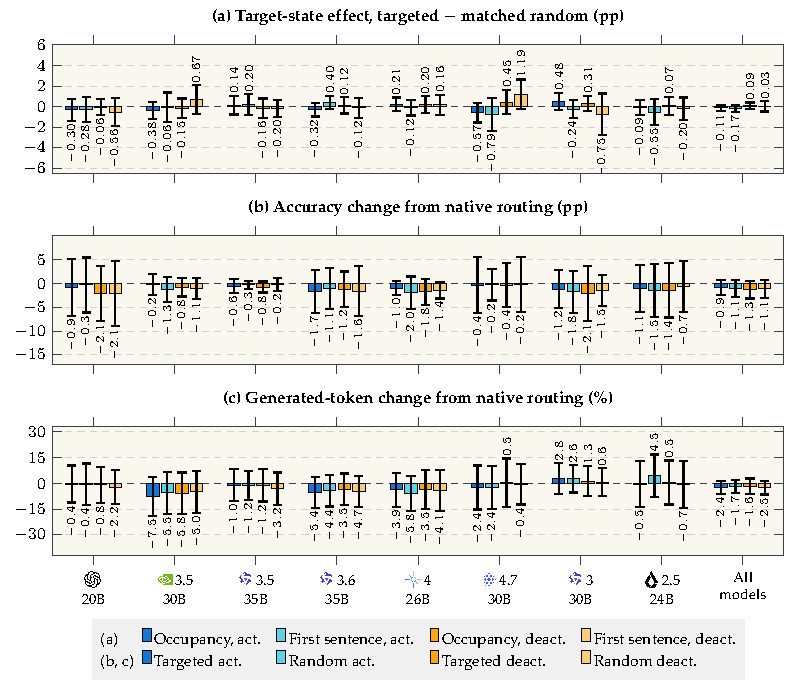
\includegraphics[width=\linewidth]{figures/journal/routing.pdf}
\caption{Paired effects of routing interventions at central strength.
%
(a) Target-state occupancy and first-sentence state for targeted minus matched random edits, signed so that positive values favor the intended direction.
%
(b) Accuracy and (c) generated tokens to the final answer for each edited arm relative to native routing.
%
Labels give the means, and whiskers show family-bootstrap simultaneous 95\% confidence intervals within each model and contrast family.
%
The pooled group averages models and classes within each family before weighting benchmarks equally.}
\label{fig:routing}
\end{figure}

The edits also leave generation cost and answer quality unchanged.
%
Relative to matched random activation, targeted activation changes accuracy by \cid{0.20}{0.87}{0.87} pp and generated tokens by \cid{-0.7}{2.1}{2.1}\%.
%
Relative to native routing, every edited arm has a lower mean accuracy, by 0.89 to 1.31 pp, and 1.6 to 2.5\% fewer generated tokens (Figure~\ref{fig:routing}).
%
Each of these intervals contains zero under the simultaneous correction across the efficiency contrasts.
%
Without that correction, the 1.31-point loss after targeted deactivation has a 95\% interval from $-2.49$ to $-0.13$ pp, so a small accuracy cost of editing cannot be excluded.
%
Appendix~\ref{app:routing-levels} reports the accuracy and token levels of every arm.
%

Native traces nevertheless associate reasoning states with the remaining solution length.
%
At the same question and absolute position, a Verify or Monitor sentence precedes shorter remaining reasoning in all seven models with saved native labels, whereas an Analyze sentence precedes longer remaining reasoning in all seven (Appendix~\ref{app:efficiency-link}).
%
Before any intervention outcome existed, we pre-registered the prediction that the token effect of each model--class edit would follow the sign and rank of this native association.
%
The measured token effects do not follow it: their Spearman correlation with the native associations across 49 model--class cells is $-0.11$, with a 95\% interval from $-0.29$ to $0.13$, and the signs agree in 41\% of the 41 signed cells.
%
The corresponding accuracy correlation is $0.07$, from $-0.16$ to $0.31$.
%
A state that accompanies shorter native solutions therefore does not shorten generation when its nominated experts are activated.
%

A stronger exploratory edit leaves the same conclusion.
%
Forcing the high-count nominated sets at all three depth regions throughout the analysis window changes target-state occupancy by \cid{0.04}{0.46}{0.46} pp relative to the matched forced controls in four models (Appendix~\ref{app:routing-strong}).
%
Both forced arms lower mean accuracy relative to native routing, by \cid{1.52}{2.18}{2.18} pp for the nominated sets and \cid{1.35}{2.37}{2.37} pp for the controls.
%
We specified this arm after inspecting the primary contrasts, so it qualifies the central result without replacing it.
%

\subsection{Sustained steering changes the computation, not the reasoning state}
\label{sec:whole-results}

Steering the efficiency-directed states throughout the reasoning makes no model reason more efficiently than matched random edits (Table~\ref{tab:whole}).
%
At full strength, the targeted composite lengthens the reasoning of GPT-OSS-20B by \cid{40.9}{31.8}{31.8}\% and lowers the accuracy of Nemotron by \cid{-10.43}{6.56}{6.56} pp and of Qwen3-30B by \cid{-14.28}{14.10}{14.10} pp, and the intervals of the other models contain zero.
%
Across all models, the composite changes reasoning tokens by \cid{-9.9}{375.6}{375.6}\% and accuracy by \cid{-8.87}{15.67}{15.67} pp, so no model meets the efficiency criterion of Section~\ref{sec:whole-steering}.
%
Relative to native routing, mean accuracy falls by 14.34 pp after targeted edits and by 5.47 pp after matched random edits.
%

The composite averages states whose effects differ in direction and size (Figure~\ref{fig:whole-states}).
%
At base strength, 8.0\% of the targeted-minus-random contrasts have simultaneous intervals that exclude zero, and each of them lengthens the reasoning or lowers accuracy.
%
Suppressing Implement lowers accuracy by \cid{-48.59}{24.96}{24.96} pp in Nemotron and by \cid{-42.88}{21.19}{21.19} pp in Qwen3-30B.
%
Suppressing Analyze lowers accuracy by \cid{-26.81}{19.89}{19.89} pp in Qwen3.6 and by \cid{-15.23}{10.92}{10.92} pp in Nemotron, whose reasoning it also lengthens by \cid{80.2}{52.8}{52.8}\%.
%
In GPT-OSS-20B at half strength, promoting Read, Analyze, Explore or Plan multiplies the reasoning length by 3.8 to 6.2 and lowers accuracy by 45.6 to 60.6 pp, in the direction of the native association of these states with longer remaining reasoning (Appendix~\ref{app:efficiency-link}).
%

The edits change the computation more than the reasoning state.
%
Against matched random edits, the occupancy of the steered state changes by a median of $-0.03$ pp of the generation allowance, and the intervals of 4.6\% of the steered cells exclude zero (Table~\ref{tab:whole-occupancy}).
%
Promoting Explore and Plan in GPT-OSS-20B raises their occupancy by 1.93 and 0.75 pp, whereas suppressing Implement in Nemotron raises the occupancy of Implement itself by 36.72 pp of the allowance.
%

Varying the number of edited pairs reveals no efficient strength (Figure~\ref{fig:whole-dose}).
%
Across all models, the composite changes reasoning tokens by \cid{-12.7}{172.3}{172.3}\%, \cid{-9.5}{250.9}{250.9}\% and \cid{-9.9}{392.9}{392.9}\% at quarter, half and full strength, while the mean accuracy change falls from $-3.40$ pp to $-6.70$ pp and $-8.87$ pp at the same strengths.
%
The pooled slope of Equation~\eqref{eq:whole-slope} is \cid{-2.73}{12.55}{12.55} accuracy points per doubling of the edited pairs, and its token slope is centered on zero.
%
Breakdown remains rare and concentrates in two models.
%
No native continuation reaches the length limit, while the share of targeted continuations that reach it rises from 0.7\% at quarter strength to 5.7\% at full strength in Nemotron and lies between 8.9\% and 10.6\% in Qwen3-30B, against at most 0.8\% in the other models.
%

% Source: report/whole-reasoning-20261021-r14/analysis-combined/EFFECTS_WHOLE.json via scripts/paper/export_whole_results.py.
\begin{table}[tb]
\centering\small
\caption{Paired effects of routing edits at full strength on reasoning tokens and strict accuracy, with family-bootstrap simultaneous 95\% confidence intervals as subscripts.
%
Targeted edits promote or suppress the efficiency-directed states of each model, random edits use matched control expert sets, and native routing is unedited; each column pair compares the first arm with the second.
%
Tokens give the percent change in reasoning tokens, with negative values meaning fewer tokens, and accuracy differences are in percentage points.
%
Intervals are simultaneous over the rows and both outcomes of each comparison and cover the outcome bounds of unfinished continuations.
%
GPT-OSS-20B and GLM-4.7-Flash ran full strength in the strength sweep.}
\label{tab:whole}
\setlength{\tabcolsep}{2.5pt}
\begin{adjustbox}{max width=\linewidth}
\begin{tabular}{@{}lcccccc@{}}
\toprule
 & \multicolumn{2}{c}{Targeted $-$ random} & \multicolumn{2}{c}{Targeted $-$ native} & \multicolumn{2}{c}{Random $-$ native} \\
\cmidrule(lr){2-3}\cmidrule(lr){4-5}\cmidrule(lr){6-7}
Model & Tokens (\%) & Acc.\ (pp) & Tokens (\%) & Acc.\ (pp) & Tokens (\%) & Acc.\ (pp) \\
\midrule
\modelname{openai}{GPT-OSS-20B} & \cid{40.9}{31.8}{31.8} & \cid{-5.81}{6.29}{6.29} & \cid{160.8}{550.3}{550.3} & \cid{-12.94}{14.15}{14.15} & \cid{85.1}{374.9}{374.9} & \cid{-7.13}{15.52}{15.52} \\
\modelname{nvidia}{Nemotron-3.5-Lightning-30B-A3B} & \cid{21.2}{59.3}{59.3} & \cid{-10.43}{6.56}{6.56} & \cid{39.7}{78.0}{78.0} & \cid{-17.07}{8.72}{8.72} & \cid{15.3}{13.4}{13.4} & \cid{-6.64}{5.89}{5.89} \\
\modelname{qwen}{Qwen3.5-35B-A3B} & \cid{20.6}{3414.3}{3414.3} & \cid{-2.19}{29.91}{29.91} & \cid{-15.0}{1521.9}{1521.9} & \cid{-7.42}{27.16}{27.16} & \cid{-29.5}{1570.7}{1570.7} & \cid{-5.22}{28.34}{28.34} \\
\modelname{qwen}{Qwen3.6-35B-A3B} & \cid{-45.8}{240.0}{240.0} & \cid{-13.69}{16.61}{16.61} & \cid{-52.1}{196.5}{196.5} & \cid{-15.69}{16.64}{16.64} & \cid{-11.6}{77.3}{77.3} & \cid{-2.00}{7.19}{7.19} \\
\modelname{gemma}{Gemma-4-26B-A4B} & \cid{-23.2}{809.1}{809.1} & \cid{-4.70}{23.61}{23.61} & \cid{-20.3}{510.0}{510.0} & \cid{-11.35}{19.29}{19.29} & \cid{3.8}{486.2}{486.2} & \cid{-6.65}{16.35}{16.35} \\
\modelname{zhipu}{GLM-4.7-Flash (30B-A3B)} & \cid{-32.3}{1573.1}{1573.1} & \cid{-13.06}{29.49}{29.49} & \cid{-11.8}{2580.1}{2580.1} & \cid{-15.94}{30.47}{30.47} & \cid{30.3}{1047.4}{1047.4} & \cid{-2.89}{19.45}{19.45} \\
\modelname{qwen}{Qwen3-30B-A3B} & \cid{7.5}{262.7}{262.7} & \cid{-14.28}{14.10}{14.10} & \cid{16.3}{295.3}{295.3} & \cid{-20.88}{16.50}{16.50} & \cid{8.2}{264.1}{264.1} & \cid{-6.60}{14.78}{14.78} \\
\modelname{liquid}{LFM2.5-24B-A2B} & \cid{-31.2}{1218.8}{1218.8} & \cid{-6.61}{28.17}{28.17} & \cid{-34.2}{547.3}{547.3} & \cid{-13.20}{23.29}{23.29} & \cid{-4.3}{258.3}{258.3} & \cid{-6.59}{15.53}{15.53} \\
\midrule
All models & \cid{-9.9}{375.6}{375.6} & \cid{-8.87}{15.67}{15.67} & \cid{-2.4}{343.7}{343.7} & \cid{-14.34}{15.08}{15.08} & \cid{8.3}{213.5}{213.5} & \cid{-5.47}{10.88}{10.88} \\
\bottomrule
\end{tabular}
\end{adjustbox}
\end{table}


\begin{figure}[tb]
\centering
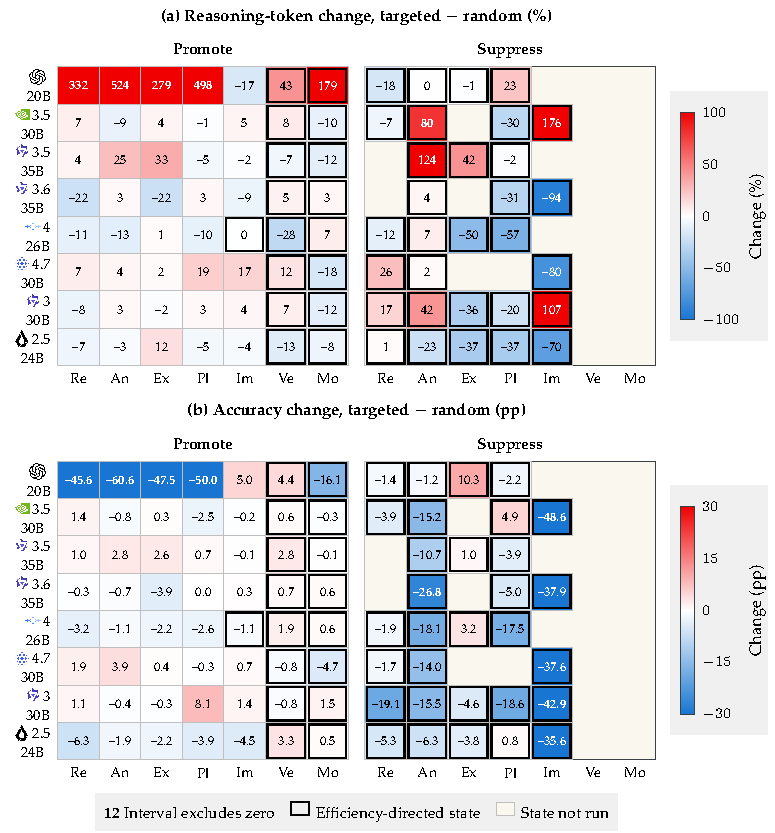
\includegraphics[width=\linewidth]{figures/journal/whole_states.pdf}
\caption{Per-state effects of steering the whole reasoning at each model's base strength, targeted against matched random edits.
%
Panel (a) gives the percent change in reasoning tokens, with negative values meaning fewer tokens, and panel (b) gives the change in strict accuracy in percentage points.
%
Rows are models, and in each panel the left block promotes a state while the right block suppresses it.
%
Re, An, Ex, Pl, Im, Ve and Mo abbreviate Read, Analyze, Explore, Plan, Implement, Verify and Monitor.
%
Blue marks a decrease and red an increase, with the color scale clipped at $\pm$100\% in (a) and $\pm$30 pp in (b), while printed values are not clipped.
%
Bold numbers have a family-bootstrap simultaneous 95\% interval, over the outcome bounds of unfinished continuations, that excludes zero.
%
Outlined cells are efficiency-directed states, and empty cells are states the model does not suppress.
%
The base strength is full except for GPT-OSS-20B and GLM-4.7-Flash, which use half strength.}
\label{fig:whole-states}
\end{figure}

\begin{figure}[tb]
\centering
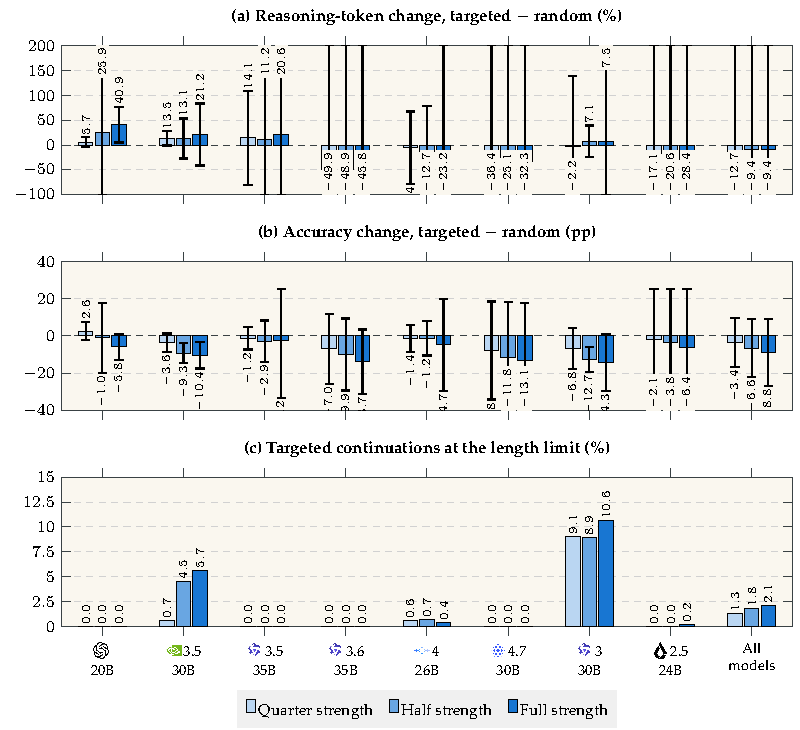
\includegraphics[width=\linewidth]{figures/journal/whole_dose.pdf}
\caption{Efficiency of steering the whole reasoning at quarter, half and full strength.
%
Panels (a) and (b) give the reasoning-token and accuracy change of targeted against matched random edits, averaged over each model's efficiency-directed states, and panel (c) gives the share of targeted continuations of these states that reach the length limit.
%
Labels give the means, and whiskers show family-bootstrap simultaneous 95\% intervals over all strengths, models and outcome bounds, cut at the panel edge when they extend beyond it.
%
The pooled group averages the models within each family before weighting benchmarks equally.}
\label{fig:whole-dose}
\end{figure}

\subsection{Promotion changes engagement without establishing control}
\label{sec:utility-results}

Historical Qwen3.6 prefix interventions increase target inclusion relative to native routing (Appendix~\ref{app:interventions}).
%
The mean intended target-inclusion fraction increases by \cid{0.1376}{0.0613}{0.0506} when two targets are promoted across eight verification families.
%
Single-pulse promotion in a second pilot increases it by \cid{0.2940}{0.1663}{0.1821}, across thirteen families covering verification and commitment transitions.
%
These are routing-engagement outcomes.
%
The larger fresh comparison leaves the semantic effect uncertain under the original simultaneous intervals and missing-judgment bounds (Appendix~\ref{app:interventions}).
%
More target inclusion does not by itself establish substantive verification.
%

Complete historical global steering does not establish a positive accuracy effect and includes harmful policies (Appendix~\ref{app:interventions}).
%
The separate candidate-recognition protocol does not qualify in five evaluated models and remains incomplete in two (Appendix~\ref{app:verification-qualification}).
%
Together with the paired continuations, these results separate a change in the selected experts from a change in the reasoning the model produces.
%
